\documentclass[12pt]{amsart}

\usepackage{a4wide, amsxtra}

\usepackage[pdftex]{graphicx}

\usepackage{hyperref}

 \title{MATH101 Assignment 9}

 \author{Mark Villar}

\begin{document} 

\maketitle 

\begin{enumerate}
	
	\item We determine the following limits using the Bernoulli-de l'H\^{o}pital Rule.
	
		\begin{enumerate}
		
			\item Since $\ln x \rightarrow -\infty$ and $x-1 \rightarrow -1$ as $x \rightarrow 0$, 
			l'H\^{o}pital's Rule cannot be applied.  Consequently, the limit fails to exist as
			$$\lim_{x \rightarrow 0} \frac{\ln x}{x-1} = \frac{-\infty}{-1} = \infty$$
			
			\item Since $(1+x)^p-1 \rightarrow 0$ and $x \rightarrow 0$ as $x \rightarrow 0$, we have an
			indeterminate form $\frac{0}{0}$. If we let $f(x)=(1+x)^p-1$ and $g(x)=x$, then $f$ and $g$ are 			both differentiable in $\mathbb{R}$ and $g'(x) \ne 0$, thus we can apply l'H\^{o}pital's Rule.
				\begin{align}
					%\lim_{x\rightarrow0} \frac{f(x)}{g(x)} & = \frac{f'(0)}{g'(0)} \notag \\
					\lim_{x\rightarrow0} \frac{(1+x)^p-1}{x} & = \lim_{x\rightarrow0} \frac{p(1+x)^{p-1}}{1} 					\notag \\
					& = p(1+0)^{p-1} = p \notag
				\end{align}
				
			\item Let $y=\left(1+\frac{4}{x}\right)^x.$ Then
				\begin{align}
					\ln y = \ln \left(1+\frac{4}{x}\right)^x \notag & = x \ln \left(1+\frac{4}{x}\right) \notag \\
					& = \frac{\ln \left(1+\frac{4}{x}\right)}{\frac{1}{x}} \notag
				\end{align}
			
			Since $\ln\left(1+\frac{4}{x}\right) \rightarrow 0$ and $\frac{1}{x} \rightarrow 0$ as $x
			\rightarrow \infty$, we have indeterminate form $\frac{0}{0}$. As the conditions for applying 
			l'H\^{o}pital's Rule are met for $x>0$, it follows that
				\begin{align}
					\lim_{x\rightarrow\infty} \frac{\ln \left(1+\frac{4}{x}\right)}{\frac{1}{x}} & = 
					\lim_{x\rightarrow\infty} \frac{\left(\frac{1}{1+\frac{4}{x}}\right)\left(-\frac{4}{x^2}\right)}
					{-\frac{1}{x^2}} \notag \\
					& = \lim_{x\rightarrow\infty} \frac{4}{1+\frac{4}{x}} = 4 \notag \\
					& = \lim_{x\rightarrow\infty} \ln y \notag 
				\end{align}
			As the natural logarithm function is continuous,
				\begin{align}
					\lim_{x\rightarrow\infty} \ln y & = \ln\left(\lim_{x\rightarrow\infty} y\right) = 4 \notag \\
					& \Rightarrow \lim_{x\rightarrow\infty} y = e^4 \notag \\
					& \Rightarrow \lim_{x\rightarrow\infty} \left(1+\frac{4}{x}\right)^x = e^4 \notag
				\end{align}
				
			\item Since $\sin x - x \rightarrow 0$ and $x^3 \rightarrow 0$ as $x \rightarrow 0$, we have an
			indeterminate form $\frac{0}{0}$. If we let $j(x)=\sin x - x$ and $k(x)=x^3$, then $j$ and $k$ 				are both differentiable in $\mathbb{R}$ and $k'(x) \ne 0$ (except at $x=0$). Thus we can apply 
			l'H\^{o}pital's Rule. 
				\begin{align}
					\lim_{x\rightarrow0} \frac{\sin x-x}{x^3} = \lim_{x\rightarrow0} \frac{\cos x-1}{3x^2}
					\notag
				\end{align}
			Since $\cos x-1 \rightarrow 0$ and $3x^2 \rightarrow 0$ as $x \rightarrow 0$, we again have
			an indeterminate form and thus can apply l'H\^{o}pital's Rule a second time.	
				\begin{align}
					\lim_{x\rightarrow0} \frac{\cos x-1}{3x^2} = \lim_{x\rightarrow0} \frac{-\sin x}{6x}							\notag
				\end{align}
			This limit is indeterminate form $\frac{0}{0}$ once again so a third application of l'H\^{o}pital's 				Rule is required.
				\begin{align}
					\lim_{x\rightarrow0} \frac{-\sin x}{6x}	& = \lim_{x\rightarrow0} \frac{-\cos x}{6} = 
					-\frac{1}{6} \notag
				\end{align}
				
		\end{enumerate}
	\bigskip	
	\item For $f: \mathbb{R} \longrightarrow \mathbb{R}, \hspace{0.3cm} x\longmapsto-\frac{2x^2}{1+x^2}$ \\
		As $f$ is differentiable everywhere and its domain has no endpoints, then
			\begin{align}
				f'(x)&=\frac{(1+x^2)(-4x)-(-2x^2)(2x)}{(1+x^2)^2}=\frac{-4x-4x^3+4x^3}{(1+x^2)^2}=
				-\frac{4x}{(1+x^2)^2} \notag \\
				f''(x)&=\frac{(1+x^2)^2(-4)-(-4x)(2)(1+x^2)(2x)}{(1+x^2)^4}=
				\frac{(1+x^2)(-4)+(8x)(2x)}{(1+x^2)^3} \notag \\
				&=\frac{-4-4x^2+16x^2}{(1+x^2)^3}=\frac{12x^2-4}{(1+x^2)^3}=
				\frac{4(3x^2-1)}{(1+x^2)^3} \notag 
			\end{align}
			
		\begin{enumerate}
		
			\item 
				\begin{align}
					f'(x)&=-\frac{4x}{(1+x^2)^2}=0 \hspace{0.3cm} \text{if and only if} \hspace{0.3cm}x=0					\notag \\
					f''(0)&=\frac{0-4}{(1+0)^3}=-\frac{4}{1}=-4 < 0 \notag \\
					f(0) & = -\frac{0}{1+0} = 0 \notag
			\end{align}
			
			Thus there is only one critical point at $x=0$, which is an absolute maximum.
			\item 
				\begin{align}
					f'(x)=
					\begin{cases}
						< 0 \hspace{0.3cm} \text{for} \hspace{0.3cm} x>0 \notag \\
						= 0 \hspace{0.3cm} \text{for} \hspace{0.3cm} x=0 \notag \\
						> 0 \hspace{0.3cm} \text{for} \hspace{0.3cm} x<0 \notag
					\end{cases}
				\end{align}
			
			Thus $f$ is increasing when $x<0$ while it is decreasing when $x>0$.
			\item 
				\begin{align}
					f''(x)=
					\begin{cases}
						< 0 \hspace{0.3cm} \text{for} \hspace{0.3cm} \left(-\frac{\sqrt{3}}{3},
						\frac{\sqrt{3}}{3}\right) \notag \\
						= 0 \hspace{0.3cm} \text{for} \hspace{0.3cm} x=-\frac{\sqrt{3}}{3}, 
						\frac{\sqrt{3}}{3} \notag \\
						> 0 \hspace{0.3cm} \text{for} \hspace{0.3cm}\left(-\infty,-\frac{\sqrt{3}}{3}\right)
						\hspace{0.3cm} \text{and} \hspace{0.3cm} \left(\frac{\sqrt{3}}{3},\infty\right) 							\notag
					\end{cases}
				\end{align}
				
			Thus $f$ is concave down when $-\frac{\sqrt{3}}{3}<x<\frac{\sqrt{3}}{3}$ while it is concave up 
			when $x<-\frac{\sqrt{3}}{3}$ and $x>\frac{\sqrt{3}}{3}$. It has inflection points at 
			$x=-\frac{\sqrt{3}}{3}, \frac{\sqrt{3}}{3}$ (which are approximately $-0.58$ and $0.58$ 					respectively). \\
			
			\item Since $2x^2 \rightarrow \infty$ and $1+x^2 \rightarrow \infty$ as $x \rightarrow \infty$, we 			have an indeterminate form $\frac{\infty}{\infty}$. As both functions are differentiable in 
			$\mathbb{R}$, we apply l'H\^{o}pital's Rule twice to evaluate the following limits,
				\begin{align}
					\lim_{x\rightarrow \infty} -\frac{2x^2}{1+x^2}=-\lim_{x\rightarrow \infty} 
					\frac{2x^2}{1+x^2}=-\lim_{x\rightarrow \infty} \frac{4x}{2x}= 
					-\lim_{x\rightarrow \infty} \frac{4}{2} = -2 \notag \\
					\lim_{x\rightarrow -\infty} -\frac{2x^2}{1+x^2}=-\lim_{x\rightarrow-\infty}
					\frac{2x^2}{1+x^2}=-\lim_{x\rightarrow-\infty} \frac{4x}{2x} =  										-\lim_{x\rightarrow -\infty} \frac{4}{2} = -2 \notag
				\end{align}
			\\
			Thus $f\rightarrow-2$ as $x \rightarrow\pm\infty$.  Geometrically, $f$ has an horizontal 
			asymptote at $y=-2$. We sketch the graph of $f$ below.
				\begin{figure}[h]
					\centering
					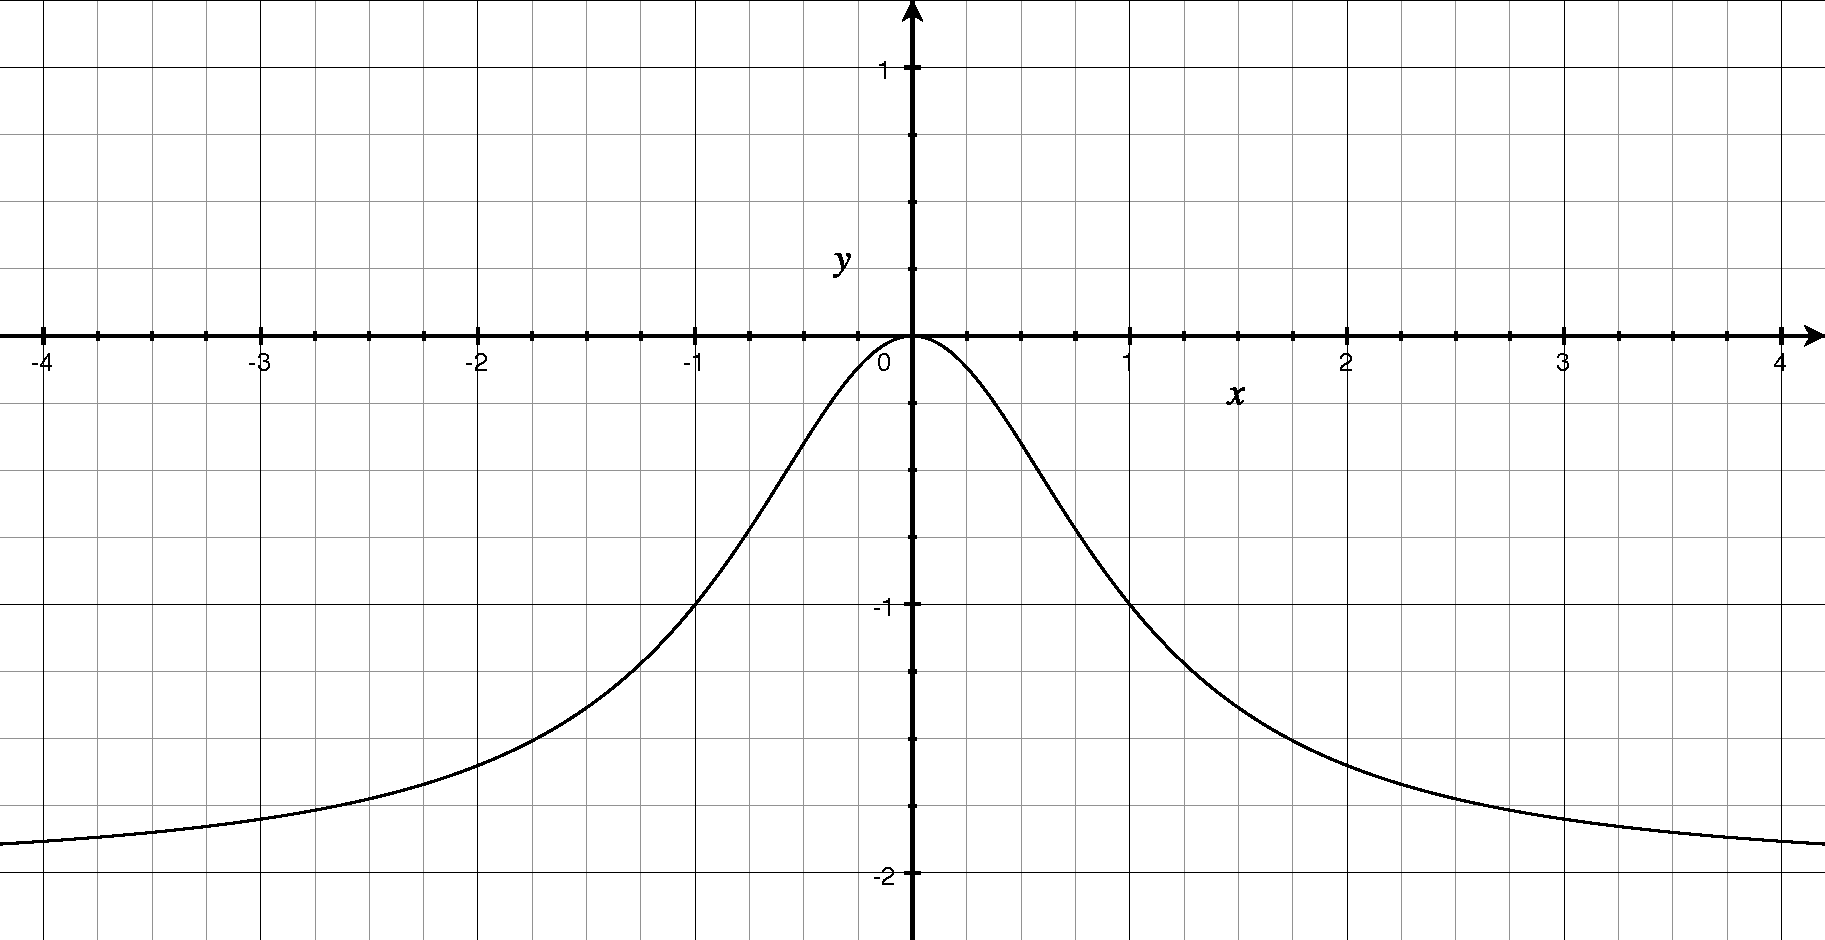
\includegraphics[width=5in]{2f.pdf}
				\end{figure} \\
		\end{enumerate}
								
	\item For $f: \mathbb{R} \longrightarrow \mathbb{R}, \hspace{0.3cm} x\longmapsto 
		e^{-\frac{(x-\mu)^2}{\sigma^2}} \hspace{0.3cm} \text{with} \hspace{0.3cm} \mu, \sigma \in 
		\mathbb{R} \hspace{0.3cm} \text{and} \hspace{0.3cm} \sigma > 0$ \\
		Since $f$ is an exponential function it is differentiable everywhere. Moreover, its domain has no 			boundary points. If we define 
		$$u:\mathbb{R}\longrightarrow\mathbb{R}, \hspace{0.3cm} x \longmapsto
		-\frac{(x-\mu)^2}{\sigma^2}, \hspace{0.3cm} \text{then}$$
			\begin{align}
				f'(x)&= \frac{ d}{du} \left(e^u\right) \cdot \frac{ d}{dx} \left(u\right)=e^u
				\left(-\frac{2(x-\mu)}{\sigma^2}\right) = 
				-\frac{2(x-\mu) \hspace{0.05cm} e^{-\frac{(x-\mu)^2}{\sigma^2}}}{\sigma^2} 
				\notag \\
				&=-\frac{2(x-\mu)}{\sigma^2} f \notag \\
				f''(x)&= \frac{ d}{dx} \left(\frac{-2(x-\mu)}{\sigma^2}\right) f + \left(\frac{-2(x-\mu)}{\sigma^2} 				\right) f' = -\frac{2}{\sigma^2} f - \frac{2(x-\mu)}{\sigma^2} f' \notag \\
				&=-\frac{2f}{\sigma^2} - \left(\frac{2(x-\mu)}{\sigma^2}\right) 
				\left(-\frac{2(x-\mu)}{\sigma^2} f \right) = -\frac{2f}{\sigma^2} + \frac{4(x-\mu)^2}{\sigma^4} f 				\notag \\
				&= \frac{4(x-\mu)^2 \hspace{0.1cm} e^{-\frac{(x-\mu)^2}{\sigma^2}}}{\sigma^4} - 
				\frac{2 \hspace{0.1cm} e^{-\frac{(x-\mu)^2}{\sigma^2}}}{\sigma^2} \notag
			\end{align}
		
		\begin{enumerate}
		
			\item 
				\begin{align}
					f'(x)&=-\frac{2(x-\mu) \hspace{0.05cm} e^{-\frac{(x-\mu)^2}{\sigma^2}}}{\sigma^2} 
 					\hspace{0.3cm} \text{if and only if} \hspace{0.3cm} x=\mu \notag \\
					f''(\mu)&= \frac{4(0)^2 \hspace{0.1cm} e^0}{\sigma^4} - 
					\frac{2 \hspace{0.1cm} e^0}{\sigma^2}=-\frac{2}{\sigma^2}<0 \notag \\
					f(\mu)&=e^0=1 \notag
				\end{align} 
					
			Thus there is only one critical point at $x=\mu$, which is an absolute maximum.
																
			\item 
				\begin{align}
					f'(x)=
					\begin{cases}
						< 0 \hspace{0.3cm} \text{for} \hspace{0.3cm} x>\mu \notag \\
						= 0 \hspace{0.3cm} \text{for} \hspace{0.3cm} x=\mu \notag \\
						> 0 \hspace{0.3cm} \text{for} \hspace{0.3cm} x<\mu \notag
					\end{cases}
				\end{align}
				
			Thus $f$ is increasing when $x<\mu$ while it is decreasing when $x>\mu$.
			
			\item 
				\begin{align}
					& \frac{4(x-\mu)^2 \hspace{0.1cm} e^{-\frac{(x-\mu)^2}{\sigma^2}}}{\sigma^4} - 
					\frac{2 \hspace{0.1cm} e^{-\frac{(x-\mu)^2}{\sigma^2}}}{\sigma^2}=0 \notag \\
					& \frac{4(x-\mu)^2 \hspace{0.1cm} e^{-\frac{(x-\mu)^2}{\sigma^2}}}{\sigma^4} =
					\frac{2 \hspace{0.1cm} e^{-\frac{(x-\mu)^2}{\sigma^2}}}{\sigma^2} \notag \\
					& \frac{2(x-\mu)^2}{\sigma^2}=1 \Rightarrow x = \mu \hspace{0.1cm} \pm 
					\frac{1}{\sqrt{2}} \hspace{0.1cm} \sigma \notag
				\end{align}
				\begin{align}
					f''(x)=
					\begin{cases}
						< 0 \hspace{0.3cm} \text{for} \hspace{0.3cm} \left(\mu \hspace{0.1cm} - 
						\frac{1}{\sqrt{2}} \hspace{0.1cm} \sigma, \hspace{0.1cm} \mu \hspace{0.1cm} + 
						\frac{1}{\sqrt{2}} \hspace{0.1cm} \sigma \right) \notag \\
						= 0 \hspace{0.3cm} \text{for} \hspace{0.3cm} x=\mu \hspace{0.1cm} - 
						\frac{1}{\sqrt{2}} \hspace{0.1cm} \sigma, \hspace{0.1cm} \mu \hspace{0.1cm} + 
						\frac{1}{\sqrt{2}} \hspace{0.1cm} \sigma \notag \\
						> 0 \hspace{0.3cm} \text{for} \hspace{0.3cm}\left(-\infty,\hspace{0.1cm} \mu 							\hspace{0.1cm} - \frac{1}{\sqrt{2}} \hspace{0.1cm} \sigma\right) \hspace{0.3cm} 						\text{and} 	\hspace{0.3cm} \left(\mu \hspace{0.1cm} + \frac{1}{\sqrt{2}} 
						\hspace{0.1cm} \sigma,\hspace{0.1cm} \infty\right) \notag
					\end{cases}
				\end{align}
				
			Thus $f$ is concave down when $\mu\hspace{0.1cm}-\frac{1}{\sqrt{2}}\hspace{0.1cm}\sigma 				<x<\mu \hspace{0.1cm}+\frac{1}{\sqrt{2}} \hspace{0.1cm} \sigma$ while it is concave up when 			$x< \mu \hspace{0.1cm} - \frac{1}{\sqrt{2}}\hspace{0.1cm} \sigma$ and $x>\mu \hspace{0.1cm}			+\frac{1}{\sqrt{2}} \hspace{0.1cm}\sigma$.\\

			\item
			Since $f$ is an exponential function $f(x)>0$.  Geometrically, $f$ has an horizontal 
			asymptote at $y=0$. We sketch the graph of $f$ for $\mu=0$ and $\sigma=1$.							\begin{figure}[h]
					\centering
					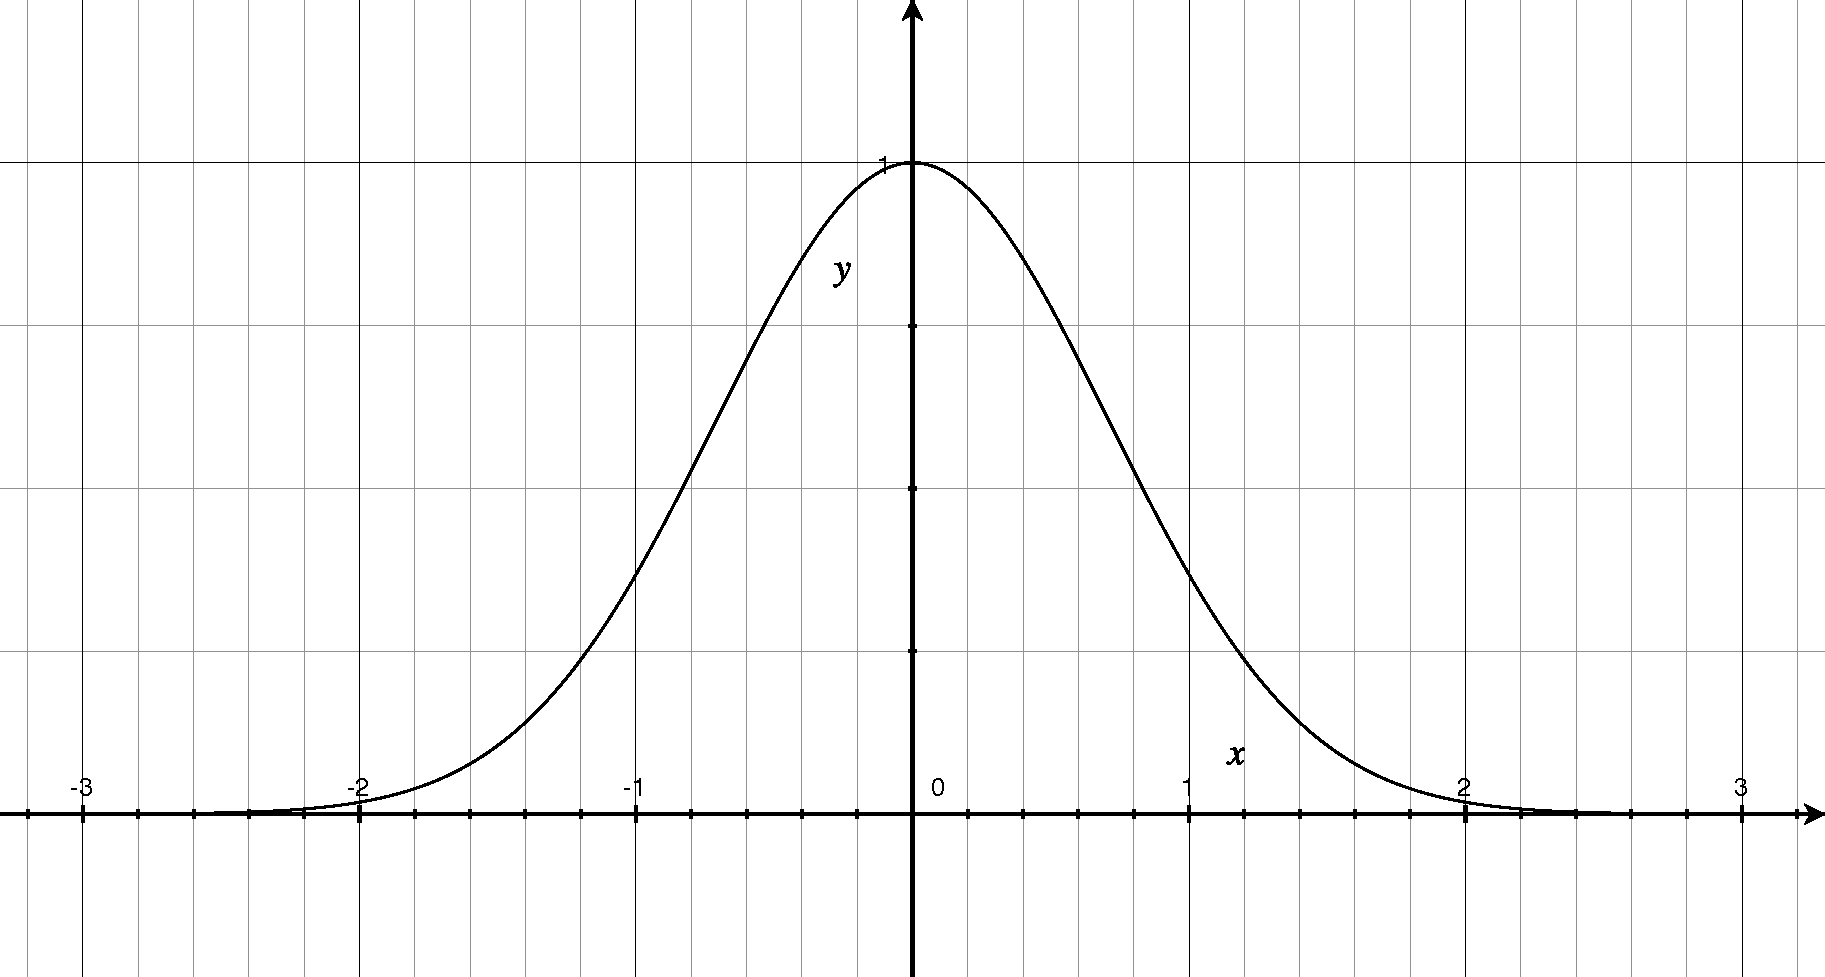
\includegraphics[width=5in]{3f.pdf}
				\end{figure} \\
			Its inflection points occur at $x=-\frac{1}{\sqrt{2}}, \frac{1}{\sqrt{2}}$ (which are approximately 				$-0.71$ and $0.71$ respectively).  \\
		
		\end{enumerate}
	
	\item Let $x$ be the length of one side of a square and $r$ be the radius of a circle. Since a cube is 			made up of six identical square faces its surface area is $6x^2$. Meanwhile, the surface area of a
		sphere is given by $4\pi r^2$. If there is only enough silver to coat 1 square metre of surface area
		for both solids, we can write 
		$$A = 6x^2 + 4\pi r^2 \le 1$$ 
		Furthermore, the volume of the two solids can be expressed as
		$$V = x^3 + \frac{4}{3} \pi r^3$$
		Assuming we use the entire 1 square metre of silver, then
		$$6x^2+4\pi r^2 = 1 \Rightarrow r=\pm \hspace{0.1cm} \frac{1}{2} \hspace{0.1cm}
		\sqrt{\frac{1-6x^2}{\pi}}$$
		As $r \ge 0$ we can rule out the negative value of $r$.  Moreover, since $1-6x^2 \ge 0$ then $0\le x 		\le \frac{1}{\sqrt{6}}$. To determine the what values of $x$ and $r$ will maximise (minimise) $V,$ 			we carry out the following algebraic steps. 
		$$V = x^3+ \frac{4}{3} \hspace{0.1cm} \pi \left(\frac{1}{2} \hspace{0.1cm} 
		\sqrt{\frac{1-6x^2}{\pi}} \right)^3= x^3 + \frac{\left(1-6x^2\right)^{\frac{3}{2}}}{6\sqrt{\pi}}$$
			\begin{align}
				V'(x) & = 3x^2 + \left(\frac{1}{6\sqrt{\pi}} \right) \left(\frac{3}{2}\right) \left(1-6x^2\right)^
				{\frac{1}{2}}\left(-12x\right) \notag \\
				& = 3x^2 - \frac{3x \hspace{0.1cm} \sqrt{1-6x^2}}{\sqrt{\pi}} = 0 \hspace{0.3cm} \text{if and 				only if} \hspace{0.3cm} x \in \left\{0,\hspace{0.1cm} \pm \hspace{0.1cm} 
				\frac{1}{\sqrt{\pi+6}}\right\} \notag
			\end{align}
		While it is clear to see that $V'(x)=0$ when $x=0$, the other roots required the following
		calculations. 
			\begin{align}
				3x^2 \hspace{0.1cm} \sqrt{\pi} & = 3x \hspace{0.1cm} \sqrt{1-6x^2} \notag \\
				x \hspace{0.1cm} \sqrt{\pi} & = \sqrt{1-6x^2} \notag \\
				x^2 \pi & = 1-6x^2 \notag \\
				1 & = (\pi+6) \hspace{0.1cm} x^2 \notag \\
				x & = \pm \hspace{0.1cm} \frac{1}{\sqrt{\pi+6}} \notag
			\end{align}
		Since $0\le x \le \frac{1}{\sqrt{6}}$ we can also rule out the negative value of $x$. We now perform 	 		the second derivative test on $x=0, \frac{1}{\sqrt{\pi+6}}$.
			\begin{align}
				V''(x)&=6x-\frac{3}{\sqrt{\pi}}\left(1-6x^2\right)^{\frac{1}{2}}-\frac{3x}{\sqrt{\pi}}
				\left(\frac{1}{2}\right)\left(1-6x^2\right)^{-\frac{1}{2}}\left(-12x\right) \notag \\
				&=6x-\frac{3 \hspace{0.1cm} \sqrt{1-6x^2}}{\sqrt{\pi}}+\frac{18x^2}{\sqrt{\pi} 
				\hspace{0.1cm} \sqrt{1-6x^2}} \notag \\
				V''(0)&=0-\frac{3}{\sqrt{\pi}}+0 = -\frac{3}{\sqrt{\pi}} < 0 \notag \\
				V''\left(\frac{1}{\sqrt{\pi+6}}\right)&=\frac{6}{\sqrt{\pi+6}}-\frac{3\hspace{0.1cm}
				\sqrt{1-\frac{6}{\pi+6}}}{\sqrt{\pi}}+\frac{\frac{18}{\pi+6}}{\sqrt{\pi} \hspace{0.1cm} 
				\sqrt{1-\frac{6}{\pi+6}}} \notag \\
				&=\frac{6}{\sqrt{\pi+6}}-\frac{3\hspace{0.1cm}\sqrt{\frac{\pi}{\pi+6}}}{\sqrt{\pi}}+
				\frac{18}{(\pi+6) \hspace{0.1cm} \sqrt{\pi} \hspace{0.1cm}\sqrt{\frac{\pi}{\pi+6}}} \notag \\
				&=\frac{6}{\sqrt{\pi+6}}-\frac{3}{\sqrt{\pi+6}}+\frac{18}{\pi \hspace{0.1cm} \sqrt{\pi+6}} 					\notag \\
				&=\frac{3}{\sqrt{\pi+6}}+\frac{18}{\pi \hspace{0.1cm} \sqrt{\pi+6}}=
				\frac{3\pi+18}{\sqrt{\pi} \hspace{0.1cm} \sqrt{\pi+6}} > 0 \notag
			\end{align} 
		Thus $x=0$ is a relative maximum while $x=\frac{1}{\sqrt{\pi+6}}$ is a relative minimum. The 
		dimensions required to maximise the total volume of the solids are therefore
		$$x=0, \hspace{0.3cm} r=\frac{1}{2} \hspace{0.1cm} \sqrt{\frac{1-0}{\pi}}=\frac{1}{2\hspace{0.1cm}
		\sqrt{\pi}}$$
		\\
		Hence the maximum volume that the silvered sphere alone can hold is given by
			\begin{align}
				V(0)=0+\frac{4}{3} \hspace{0.1cm} \pi\left(\frac{1}{2\hspace{0.1cm}\sqrt{\pi}}\right)^3=
				\frac{1}{6\sqrt{\pi}} \notag
			\end{align}
		To minimise the total volume the solids can hold, we can simply set the dimensions to $x=0$ and 
		$r=0$ such that $V=0$.
		\medskip
		\\
		However, if we were considering only non-zero solutions (at least one solid is coated with silver) 			and as such $V>0,$ then the dimensions required for a minimum are
		$$x=\frac{1}{\sqrt{\pi+6}}, \hspace{0.3cm} r=\frac{1}{2} \hspace{0.1cm} 
		\sqrt{\frac{\frac{\pi}{\pi+6}}{\pi}}=\frac{1}{2\hspace{0.1cm}\sqrt{\pi+6}}$$
		\\
		The volume given by these dimensions is given by
			\begin{align}
				V\left(\frac{1}{\sqrt{\pi+6}}\right)=\left(\frac{1}{\sqrt{\pi+6}}\right)^3+\frac{4}{3}
				\hspace{0.1cm} \pi \left(\frac{1}{2\hspace{0.1cm}\sqrt{\pi+6}}\right)^3=
				\frac{1}{6\hspace{0.1cm}\sqrt{\pi+6}} \notag
			\end{align}
		\\
		This confirms our answer as $V(0)>V\left(\frac{1}{\sqrt{\pi+6}}\right)$.
	
\end{enumerate}
	
\end{document}